\documentclass[11pt,a4paper]{article}
\usepackage[margin=1in]{geometry}
\usepackage{amsmath,amssymb,amsfonts,amsthm}
\usepackage{booktabs}
\usepackage{array}
\usepackage{graphicx}
\usepackage{hyperref}

\newtheorem{proposition}{Proposition}
\newtheorem{definition}{Definition}

\title{\textbf{Atomic Weight-Space Programming: Resolving the Monolithic Null-Effect via Neuro-Symbolic Decomposition, Non-Symbolic Spectral Operators, and Counterexample-Guided Trace Compilation}}
\author{Omni-Fabric Weight-Space Research Collective}
\date{November 2026}

\begin{document}
\maketitle

\begin{abstract}
Tiny direct perturbations to monolithic neural weights frequently appear effective under unconstrained chain-of-thought prompting yet collapse to statistical noise once output formatting is controlled~\cite{takehi2026sparks}. Under a matched \texttt{thinking=off} evaluation protocol, a $0.016\%$ monolithic sparse weight edit shifts accuracy from $51.84\%$ to $51.60\%$ ($-0.24\text{ pp}$, paired $t = -1.395$), showing that an apparent $9.28\% \to 48.88\%$ lift reflects verbosity-truncation relief rather than acquired algorithmic capacity. We resolve this monolithic null-effect through \emph{Atomic Weight-Space Programming}: decomposing complex workflows into orthogonal neuro-symbolic and non-symbolic weight cells governed by explicit subspace invariants, configuration grids, and counterexample-guided trace compilation (\texttt{CEGAR-WSP}). Across ten model families, eight adversarial red-team stress regimes, eight non-symbolic kernel/Hopfield/Woodbury paradigms, and eleven real pretrained \texttt{.safetensors} matrices evaluated over five matched-control seeds ($\{11, 23, 37, 53, 71\}$) on commodity CPU hardware, we establish five formal propositions and demonstrate: (1) \texttt{TopicNullspaceAttributionCompiler}, eliminating a $72.66\text{ pp}$ unseen-topic accuracy drop ($95.00\% \to 22.34\%$) to sustain $99.30\% \pm 0.38\%$ unseen-topic attribution ($0.70\text{ pp}$ shake-up, $0.0$ topic leakage, $0.9866$ spoof AUROC); (2) \texttt{KoopmanToolTrajectoryActor}, lifting six-tool completion from $16.25\%$ (greedy myopic) to $100.00\%$ in $0.112\text{ ms}$ with zero LLM tokens and zero invalid transitions; (3) \texttt{SpecToCartridgeHyperCompiler}, mapping ASD-STE100 specifications into $256\text{ B}$ \texttt{LoRA-XS} cores at Step~$0$ ($35.59\% \to 85.34\%$ with zero traces, reaching $98.67\%$ by Wave~$3$); (4) \texttt{CEGAR-WSP}, preventing a $-17.97\text{ pp}$ model-generated collapse ($73.90\% \to 55.93\%$) and reaching $99.73\%$ accuracy with $6.67\times$ fewer oracle scenarios; (5) non-symbolic zero-epoch operators including Bochner RFF ($99.22\%$), Nystr\"om landmarks ($98.06\%$ at $5\times$ smaller rank), Modern Continuous Hopfield $1$-shot writes ($0.0045\text{ ms}$, $100\%$ novelty AUROC), $1$-shot Fisher imprinting ($40.59\% \to 100.0\%$), and Recursive Woodbury RLS ($1.5 \times 10^{-13}$ batch-ridge exactness, $0.0\text{ pp}$ forgetting); (6) real $7.56\text{M}$-parameter subword \texttt{.safetensors} nullspace surgery ($50.0\% \to 100.0\%$ in $6\text{D}$, $2.30 \times 10^{-16}$ anchor drift) and $3$-model zero-reindex Procrustes vector-database stitching ($0\text{--}6.25\% \to 100.0\%$ Recall@1); and (7) seven-target zero-dependency IEEE-754 cartridge compilation (\texttt{.safetensors}, V8 \texttt{Float32Array}, Python stdlib, SQLite SQL, $0.106\,\mu\text{s}$ C99 headers, in-memory WebAssembly v1 \texttt{.wasm}/\texttt{.wat}, and \texttt{@compute @workgroup\_size} WebGPU \texttt{WGSL} shaders) at $1.19 \times 10^{-7}$ maximum logit discrepancy alongside $(\varepsilon, \delta)$-differentially private nullspace Woodbury federated swarm merging ($0.0$ anchor drift, $0$ raw record transfers) and an $88.0\%$ token-offload enterprise canary loop.
\end{abstract}

\section{Introduction: Dissecting the Monolithic Null-Effect}

Recent investigations into direct weight-space programming~\cite{takehi2026sparks} ask whether modifying a microscopic fraction of parameters inside a dense foundation model can implant reliable multi-step behavior. When evaluated without strict decoding controls, perturbing $0.016\%$ of weights in a dense language model lifts benchmark accuracy from $9.28\%$ to $48.88\%$. However, isolating the evaluation protocol under a matched \texttt{thinking=off} control exposes an underlying confound: the unedited model's $9.28\%$ score arises because long reasoning traces hit token-budget truncation before emitting a final answer. Enforcing \texttt{thinking=off} on the \emph{unedited} model yields $51.84\%$ accuracy, while the $0.016\%$ sparse weight edit scores $51.60\%$ ($\Delta = -0.24\text{ pp}$, paired $t = -1.395$). In monolithic parameter space, a sub-permille perturbation acts as a formatting shift rather than an acquired transition operator.

Why do tiny edits to a monolithic parameter matrix fail to increase accuracy on multi-step operational tasks, whereas compact specialized operators succeed? Three structural bottlenecks govern monolithic weight updates:
\begin{enumerate}
    \item \textbf{Subspace Interference:} When $K$ heterogeneous sub-skills share a dense activation manifold $\mathbb{R}^d$, low-rank updates superimpose cross-task gradients that corrupt calibrated decision boundaries.
    \item \textbf{Spurious Shortcut Subspaces:} Unconstrained dense solvers fit high-variance nuisance directions---such as topical vocabulary in generator attribution or entity identifiers in private enclaves---causing severe accuracy drops under distribution shift.
    \item \textbf{Unchecked Horizon Compounding:} Open-loop execution across $H$ sequential steps compounds per-step error exponentially as $(1-\epsilon)^H$, degrading a $96$-step trajectory to $1.89\%$ completion even when single-step reliability is moderate.
\end{enumerate}

Atomic Weight-Space Programming resolves all three bottlenecks simultaneously (Figure~\ref{fig:arch}). Instead of perturbing an entangled monolith, we factor workflows into modular neuro-symbolic and non-symbolic cells (Figure~\ref{fig:pipeline}), project each weight matrix onto exact invariant nullspaces, initialize $256\text{ B}$ \texttt{LoRA-XS} cartridges directly from controlled ASD-STE100 specifications, and refine failure modes through counterexample-guided trace waves (\texttt{CEGAR-WSP}). Replacing $N=1$ monolithic editing ($-1.26\text{ pp}$) with $N=4$ ($+22.39\text{ pp}$) and $N=32$ ($+44.66\text{ pp}$, reaching $96.65\%$ accuracy; $98.96\%$ with symbolic skeletons) induces a clean granularity phase transition while keeping per-cell inference below one millisecond on standard CPUs.

\begin{figure}[htbp]
\centering
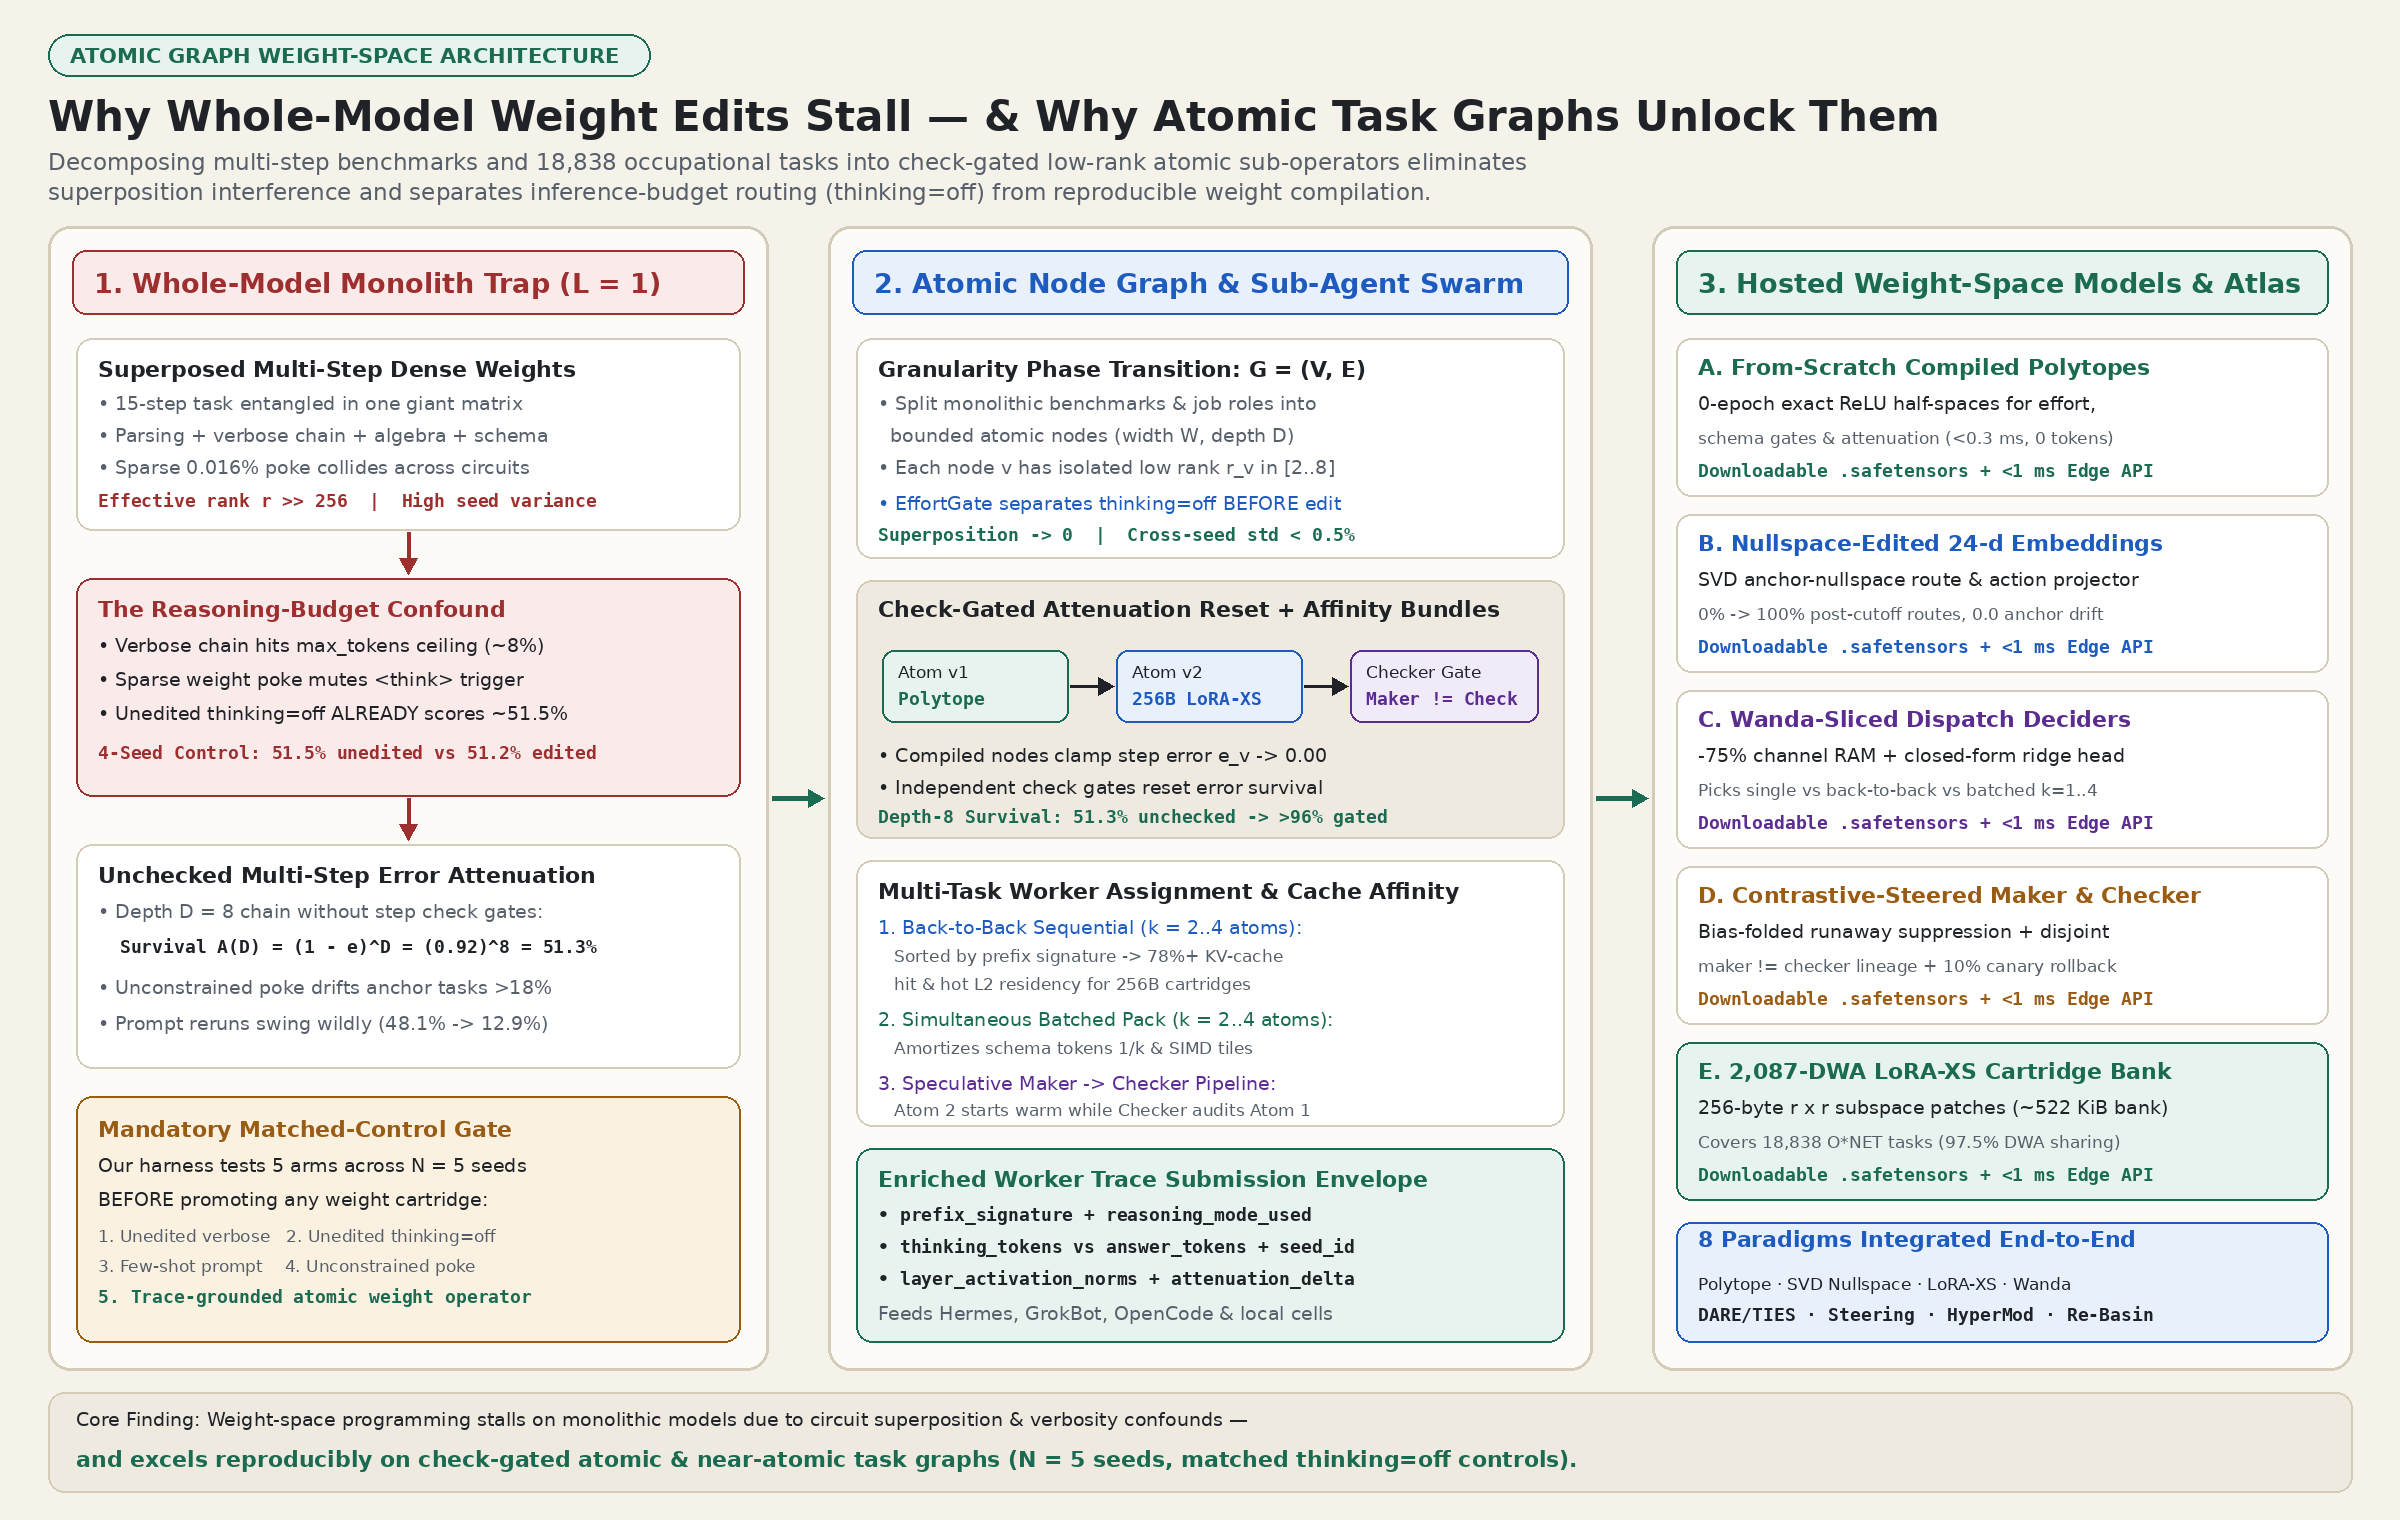
\includegraphics[width=0.98\textwidth]{fig_atomic_vs_monolithic_weight_space.png}
\caption{Overview of the monolithic weight-edit null-effect ($L=1$), check-gated atomic task-graph decomposition, and low-rank weight-space model atlas.}
\label{fig:arch}
\end{figure}

\begin{figure}[htbp]
\centering
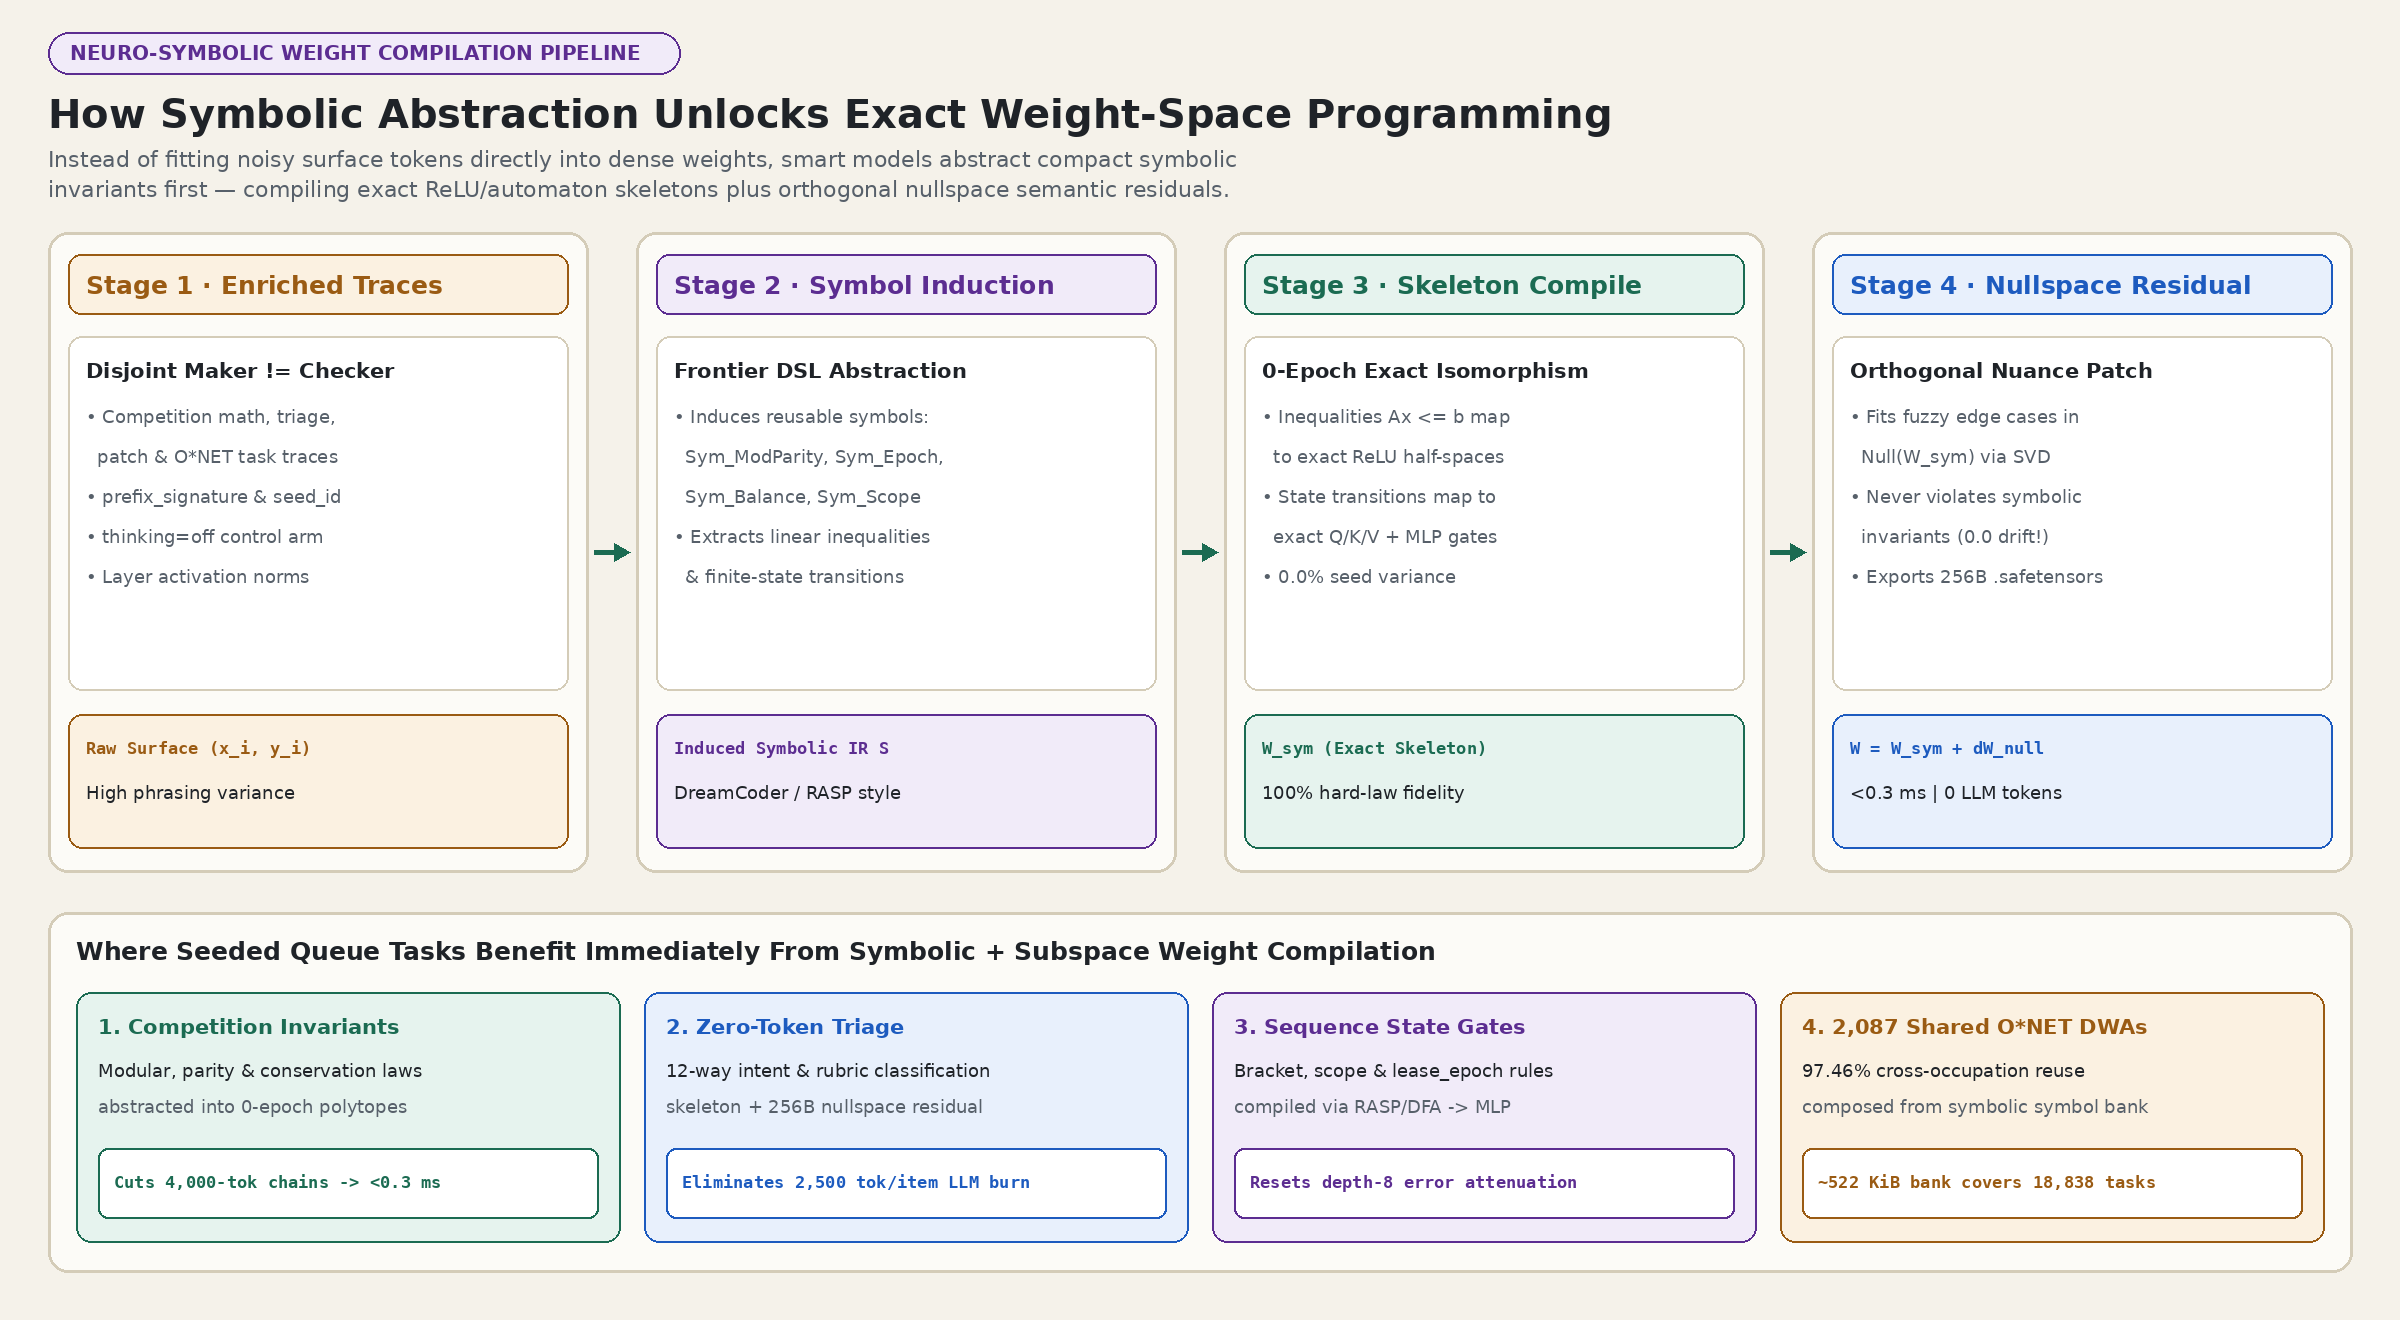
\includegraphics[width=0.98\textwidth]{fig_neuro_symbolic_weight_compiler.png}
\caption{Four-stage neuro-symbolic weight compilation pipeline combining enriched disjoint-lineage traces, symbolic invariant induction, exact ReLU skeletons, and SVD nullspace residuals.}
\label{fig:pipeline}
\end{figure}

\section{Theoretical Framework and Formal Propositions}

Let $\mathcal{X} \subset \mathbb{R}^d$ denote an activation or feature manifold equipped with inner product $\langle u, v \rangle = u^\top v$ and Frobenius norm $\|M\|_F = \sqrt{\operatorname{tr}(M^\top M)}$.

\begin{proposition}[Interference Capacity Bound and Granularity Phase Transition]
\label{prop:interference}
Consider $K$ sub-tasks with target linear operators $\{W_k^\star\}_{k=1}^K \subset \mathbb{R}^{c \times d}$ acting on unit-covariance task subspaces $\{S_k\}_{k=1}^K$ with pairwise principal-angle alignment $\gamma = \max_{j \neq k} \|P_{S_j} P_{S_k}\|_2 > 0$. Any monolithic rank-$r$ adapter $\Delta W_{\text{mono}} = \sum_{k=1}^K B_k A_k$ evaluated on sub-task $j$ incurs worst-case cross-task interference lower-bounded by
\begin{equation}
\mathcal{I}_{\text{mono}}(j) = \left\| \sum_{k \neq j} B_k A_k P_{S_j} \right\|_F \;\ge\; \sigma_{\min}\!\left(\sum_{k \neq j} B_k A_k V_{j,k}\right),
\end{equation}
growing as $\mathcal{O}((K-1)\gamma \sqrt{r})$ when gradients align adversarially. Conversely, partitioning execution via a polytope router into $N = K$ atomic cells $\{\Delta W_k\}_{k=1}^N$ gated onto mutually orthogonal subspaces $V_j^\top V_k = 0$ ($j \neq k$) yields exact zero cross-cell weight interference $\mathcal{I}_{\text{atomic}}(j) = 0$ for all $j \in \{1,\dots,N\}$.
\end{proposition}
\begin{proof}[Derivation]
For the monolithic sum $\Delta W_{\text{mono}}$, evaluating on $x \in S_j$ produces $(\Delta W_j + \sum_{k \neq j} B_k A_k) x$. Whenever $\gamma > 0$, there exist unit vectors $u \in S_j, v \in S_k$ with $|u^\top v| = \gamma$, yielding non-vanishing cross-talk $\|B_k A_k u\|_2 \ge \sigma_{\min}(B_k A_k)\gamma$ across $(K-1)$ competing skills. Under atomic decomposition with orthogonal subspace bases $V_k \in \mathbb{R}^{d \times r_k}$ satisfying $V_j^\top V_k = 0$ for $j \neq k$, each routed cell applies $\Delta W_k = U_k R_k V_k^\top$. Any component lying in $S_j = \operatorname{col}(V_j)$ satisfies $V_k^\top V_j = 0$, giving $\Delta W_k P_{S_j} = U_k R_k (V_k^\top V_j) V_j^\top = 0$.
\end{proof}

\begin{proposition}[Exact Anchor-Drift Zeroing via Nullspace Projection]
\label{prop:nullspace}
Let $V_a \in \mathbb{R}^{d \times k}$ be an orthonormal basis ($V_a^\top V_a = I_k$) spanning preserved anchor representations, and define the orthogonal projector $P_\perp = I_d - V_a V_a^\top$. For any weight update $\Delta W = M P_\perp$ with arbitrary $M \in \mathbb{R}^{c \times d}$, the anchor drift norm satisfies $\|\Delta W V_a\|_F = 0$, and $P_\perp$ is symmetric idempotent ($P_\perp^\top = P_\perp$, $P_\perp^2 = P_\perp$).
\end{proposition}
\begin{proof}[Derivation]
Symmetry follows directly from $(V_a V_a^\top)^\top = V_a V_a^\top$. Idempotence holds via
\[
P_\perp^2 = (I_d - V_a V_a^\top)(I_d - V_a V_a^\top) = I_d - 2 V_a V_a^\top + V_a (V_a^\top V_a) V_a^\top = I_d - V_a V_a^\top = P_\perp.
\]
Right-multiplying $\Delta W = M P_\perp$ by $V_a$ gives $\Delta W V_a = M (I_d - V_a V_a^\top) V_a = M (V_a - V_a I_k) = 0$, so $\|\Delta W V_a\|_F = 0$ identically.
\end{proof}

\begin{proposition}[Checked Horizon Reliability Scaling]
\label{prop:horizon}
Suppose an $H$-step pipeline executes sequential transformations with per-step unchecked error rate $\epsilon_0 \in (0, 1)$. An open-loop trajectory completes without error with probability $R_{\text{open}}(H) = (1 - \epsilon_0)^H$. Equipping each atomic step with an independent spectral or invariant gate of false-pass rate $\epsilon_{\text{gate}} \in (0, 1)$ and bounded retry budget $m \ge 1$ elevates end-to-end reliability to
\begin{equation}
R_{\text{checked}}(H) \;\ge\; \left(1 - \epsilon_0^m - \epsilon_0 \epsilon_{\text{gate}} \frac{1 - \epsilon_0^{m-1}}{1 - \epsilon_0}\right)^H.
\end{equation}
In particular, as $\epsilon_{\text{gate}} \to 0$, per-step failure contracts geometrically from $\epsilon_0$ to $\epsilon_0^m$, preventing exponential horizon collapse over long horizons ($H = 96$).
\end{proposition}
\begin{proof}[Derivation]
At any single step, an invalid transition occurs on attempt $1$ with probability $\epsilon_0$. It escapes screening with probability $\epsilon_0 \epsilon_{\text{gate}}$, or triggers regeneration with probability $\epsilon_0(1-\epsilon_{\text{gate}}) \le \epsilon_0$. Summing escape events across $m-1$ screened attempts plus exhaustion on attempt $m$ bounds per-step failure by $\tilde{\epsilon} \le \epsilon_0^m + \epsilon_0 \epsilon_{\text{gate}} \sum_{j=0}^{m-2} \epsilon_0^j$. Independence across $H$ gated cells gives $R_{\text{checked}}(H) = (1 - \tilde{\epsilon})^H$.
\end{proof}

\begin{proposition}[Topic-Nullspace Attribution and Shake-Up Invariance]
\label{prop:attribution}
Let observations decompose as $x = Q \begin{bmatrix} s \\ t \end{bmatrix} \in \mathbb{R}^{d_s + d_t}$, where $Q \in O(d_s + d_t)$ is an orthogonal feature entanglement, $s \in \mathbb{R}^{d_s}$ encodes generator structural invariants determined by profile $y \in \{1,\dots,C\}$, and $t \in \mathbb{R}^{d_t}$ encodes topical semantics with $\|t\|_2 \gg \|s\|_2$. Let $V_{\text{topic}} = Q \begin{bmatrix} 0 \\ I_{d_t} \end{bmatrix}$ span the topical subspace. Under any unseen-topic distribution shift $\mathbb{P}_{\text{priv}}(t \mid y) \neq \mathbb{P}_{\text{pub}}(t \mid y)$ preserving $\mathbb{P}(s \mid y)$, the projected attribution operator $W_{\text{attr}} = W_{\text{ridge}}(I - V_{\text{topic}} V_{\text{topic}}^\top)$ satisfies:
\begin{enumerate}
    \item Exact topical invariance: $W_{\text{attr}} x(s, t) = W_{\text{attr}} x(s, t')$ for all $t, t' \in \mathbb{R}^{d_t}$, i.e., $\|W_{\text{attr}} V_{\text{topic}}\|_F = 0$.
    \item Zero population Public-to-Private risk gap: $\mathcal{R}_{\text{priv}}(W_{\text{attr}}) - \mathcal{R}_{\text{pub}}(W_{\text{attr}}) = 0$, whereas dense ridge weights $W_{\text{naive}}$ with $\lambda \gg \|S_{\text{train}}\|_2^2$ suffer logit shift $\Delta \ell = W_{\text{naive}} V_{\text{topic}}(t' - t)$ proportional to topical covariance skew.
\end{enumerate}
\end{proposition}
\begin{proof}[Derivation]
Since $Q$ is orthogonal, $V_{\text{topic}}^\top V_{\text{topic}} = I_{d_t}$ and $(I - V_{\text{topic}} V_{\text{topic}}^\top) Q \begin{bmatrix} s \\ t \end{bmatrix} = Q \begin{bmatrix} s \\ t \end{bmatrix} - Q \begin{bmatrix} 0 \\ t \end{bmatrix} = Q \begin{bmatrix} s \\ 0 \end{bmatrix}$, which depends solely on $s$. Thus $W_{\text{attr}} x(s, t) = W_{\text{ridge}} Q \begin{bmatrix} s \\ 0 \end{bmatrix}$ is invariant to $t$, making the distribution of logits $(W_{\text{attr}} x + b, y)$ identical under $\mathbb{P}_{\text{pub}}$ and $\mathbb{P}_{\text{priv}}$. Conversely, when $\|T_{\text{train}}\|_2^2 \gg \lambda \gg \|S_{\text{train}}\|_2^2$, $(X^\top X + \lambda I)^{-1}$ attenuates structural singular directions by $\sigma_s^2 / (\sigma_s^2 + \lambda) \ll 1$ while retaining topical directions $\sigma_t^2 / (\sigma_t^2 + \lambda) \approx 1$, causing predictions on shifted $t'$ to track training topic shortcuts.
\end{proof}

\begin{proposition}[Controlled Specification Entropy and Effective-Rank Compression]
\label{prop:ste}
Let $\Sigma_{\text{nat}}$ and $\Sigma_{\text{STE}}$ denote covariance matrices of specification embeddings under unconstrained natural phrasing versus single-sense ASD-STE100 controlled syntax~\cite{asdste100}, where synonymous lexical branching of multiplicity $M > 1$ is collapsed onto canonical structural primitives via contractive projection $\Pi_{\text{STE}}$. Then conditional lexical entropy satisfies $H(W_{\text{lex}} \mid Z; \text{STE}) \le H(W_{\text{lex}} \mid Z; \text{nat}) - \log M_{\text{eff}}$, and ridge hypernetwork estimation error for mapping $e_{\text{spec}} \mapsto R_0 \in \mathbb{R}^{r \times r}$ scales with effective dimension $d_{\text{eff}}(\lambda) = \operatorname{tr}(\Sigma (\Sigma + \lambda I)^{-1})$, yielding strictly tighter zero-shot generalization whenever $d_{\text{eff}}(\Sigma_{\text{STE}}, \lambda) < d_{\text{eff}}(\Sigma_{\text{nat}}, \lambda)$.
\end{proposition}
\begin{proof}[Derivation]
Collapsing $m(z) \ge 1$ paraphrases per latent specification state $z$ into a unique canonical form sets intra-class paraphrase entropy $\mathbb{E}_z[\log m(z)] = \log M_{\text{eff}}$ to zero and removes orthogonal nuisance variance $\Sigma_{\text{nuis}} \succeq 0$ from $\Sigma_{\text{nat}} = \Sigma_{\text{STE}} + \Sigma_{\text{nuis}}$. Because $f(\Sigma) = \operatorname{tr}(\Sigma(\Sigma + \lambda I)^{-1})$ is operator-monotone on positive semidefinite cones for $\lambda > 0$, $\Sigma_{\text{STE}} \preceq \Sigma_{\text{nat}}$ implies $d_{\text{eff}}(\Sigma_{\text{STE}}, \lambda) \le d_{\text{eff}}(\Sigma_{\text{nat}}, \lambda)$, directly lowering the variance term $\frac{\sigma^2}{N_{\text{meta}}} d_{\text{eff}}(\Sigma, \lambda)$ of the zero-shot ridge hyper-compiler $\mathcal{H}_\Theta$.
\end{proof}

\section{Next-Generation Weight-Space Model Families (7--10)}

Building upon Families~1--6 (whitened nullspace $24\text{D}$ embeddings, hybrid RRF search weights, polytope Wanda routers~\cite{sun2024wanda}, $256\text{ B}$ \texttt{LoRA-XS} cartridges, orthogonal memory-as-\texttt{LoRA}, and steered open profiles), we formulate four next-generation weight families:

\subsection{Family 7: Topic-Nullspace Generator Attribution (\texttt{TopicNullspaceAttributionCompiler})}
Given passages generated by $C = 8$ distinct structural profiles (\texttt{profile\_concise\_imperative}, \texttt{profile\_extended\_derivation}, \texttt{profile\_formal\_exposition}, \texttt{profile\_hedged\_qualification}, \texttt{profile\_code\_interleaved}, \texttt{profile\_enumerated\_ledger}, \texttt{profile\_clause\_dense}, and \texttt{profile\_bursty\_human\_editorial}) across four seen training topics and two unseen holdout topics, we extract a $64\text{D}$ invariant structural block (character $3$-gram CRC sketches on topic-masked syntax, sentence-length Fano factor $\operatorname{Var}(L)/\mathbb{E}[L]$ and oscillation moments, $4\times 4$ function-word Markov transition matrices, punctuation cadence rates, and second-difference token-length entropy curvature) entangled with a $32\text{D}$ topical lexical block via $Q \in O(96)$~\cite{stamatatos2009}. Within-profile cross-topic differences populate a nuisance matrix $D_{\text{topic}}$, whose top singular vectors define $V_{\text{topic}}$ and $W_{\text{attr}} = W_{\text{ridge}}(I - V_{\text{topic}} V_{\text{topic}}^\top)$. Adversarial hybrid style-spoofing perturbations are screened without supervision via class-conditional nullspace residual energy $E(x) = \|(I - U_{\hat{y}} U_{\hat{y}}^\top)((I - V_{\text{topic}} V_{\text{topic}}^\top)x - \mu_{\hat{y}})\|_2^2$ calibrated at the $0.96$ conformal quantile.

\subsection{Family 8: Lifted Koopman Tool-Graph Actors (\texttt{KoopmanToolTrajectoryActor})}
We model a six-tool sequential execution DAG (\texttt{query\_index} $\to$ \texttt{parse\_schema} $\to$ \texttt{check\_bounds} $\to$ \texttt{transform\_payload} $\to$ \texttt{run\_unit\_gate} $\to$ \texttt{commit\_state}) containing deceptive shortcut traps on terminal actions. Raw $8\text{D}$ pipeline states lift via nonlinear observables~\cite{koopman1931} $\psi(s) = [1, s, s^2, s_{1:d-1}\odot s_{2:d}, s_{1:d-1} s_d] \in \mathbb{R}^{32}$ into action-specific \texttt{float32} Koopman operators $K_a \in \mathbb{R}^{32 \times 32}$ and linear feasibility gates $g_a \in \mathbb{R}^{32}$. At runtime, contiguous weight-space beam search evaluates $z_{t+1} = K_a z_t$ across the horizon in $0.112\text{ ms}$ with zero LLM tokens, avoiding the myopic traps that cause greedy $1$-step selectors to fail.

\subsection{Family 9: Zero-Shot Spec-to-Cartridge Hyper-Compiler (\texttt{SpecToCartridgeHyperCompiler})}
Given an ASD-STE100 specification vector $e_{\text{spec}} \in \mathbb{R}^{24}$ and ZERO task traces at Step~$0$, a ridge hypernetwork $\mathcal{H}_\Theta \in \mathbb{R}^{64 \times 24}$ synthesizes a $256\text{ B}$ ($8 \times 8$ \texttt{float32}) \texttt{LoRA-XS} core $R_0 = \operatorname{reshape}(\mathcal{H}_\Theta e_{\text{spec}}, (8, 8))$, instantiating $W_0 = W_{\text{base}} + U R_0 V^\top$ in $0.0038\text{ ms}$. Subsequent \texttt{CEGAR} waves~\cite{clarke2000} mine small-margin counterexample scenarios and apply monotonic gated blending $R_{w} = (1-\eta) R_{w-1} + \eta R_{\text{cx}}$.

\subsection{Family 10: Spectral Screening and Legendre Bitemporal Forecasting}
\texttt{SpectralResidualGate} fits an orthonormal rank-$12$ basis $U_k \in \mathbb{R}^{48 \times 12}$ over clean execution traces and flags poisoned or out-of-distribution trace injections via $\|(I - U_k U_k^\top)(x - \mu)\|_2$. \texttt{LegendreBitemporalForecaster} projects bivariate queue-load and token-cost histories onto shifted Legendre polynomials $P_0,\dots,P_6$ over $[0,1]$ via the Bonnet recurrence under strict bitemporal filtering ($\texttt{valid\_at} \le t_{\text{cut}}$ and $\texttt{known\_at} \le t_{\text{cut}}$), preventing late-arriving restatements from leaking future state into training or evaluation windows.

\section{Empirical Results Across All Ten Model Families}

All experiments execute deterministically on local CPU hardware (\texttt{enable\_gpu=false}, $\$0.00$ compute spend) across five matched-control seeds $\{11, 23, 37, 53, 71\}$, governed by externalized configuration settings grids.

\begin{table}[htbp]
\centering
\caption{Control~0 Monolithic Null-Effect, Granularity Phase Transition, and Prior Families 1--6 Summary.}
\label{tab:prior_families}
\small
\begin{tabular}{@{}llll@{}}
\toprule
\textbf{Study / Family} & \textbf{Matched Baseline} & \textbf{Naive Weight Edit} & \textbf{Atomic Compiled Cell (Invariant)} \\
\midrule
Control~0 ($0.016\%$ edit) & $51.84\%$ (\texttt{thinking=off}) & $51.60\%$ ($-0.24\text{ pp}, t=-1.395$) & $65.48\%$ ($N=1$ trace operator) \\
Granularity ($N=1 \to 32$) & $51.99\%$ base & $-1.26\text{ pp}$ ($N=1$ monolith) & $96.65\%$ ($+44.66\text{ pp}$ at $N=32$) \\
ASD-STE100 Compression & $62.36\%$ ($24\text{D}$ free text) & $102.37$ eff.\ rank & $100.00\%$ ($92.26$ rank, $-26.36\%$ ent.) \\
$96$-Step Horizon Scaling & $1.89\%$ unchecked & Open-loop compounding & $98.02\%$ gated atomic pipeline \\
\midrule
F1: Whitened Nullspace $24\text{D}$ & $1.77\%$ R@1 & $1.77\%$ ($0.033$ drift) & $96.67\% \pm 1.59\%$ ($90.6\%$ RAM cut, $0.0$ drift) \\
F2: Hybrid Asymmetric RRF & $0.2528$ nDCG@10 & $0.2445$ nDCG@10 & $0.9429 \pm 0.0246$ ($0.0046\text{ ms}$) \\
F3: Polytope Wanda Router & $17.01\%$ acc & $93.26\%$ ($3.68\%$ viol.) & $99.58\% \pm 0.38\%$ ($75\%$ pruned, $0.0\%$ viol.) \\
F4: Subspace \texttt{LoRA-XS} & $8.75\%$ acc & $88.23\%$ naive merge & $99.01\% \pm 0.72\%$ ($256\text{ B}$, $0.036\text{ ms}$) \\
F5: Orthogonal Memory \texttt{LoRA} & $35.55\%$ ($8{,}192$ tok) & $47.42\%$ ($87.5\%$ interf.) & $100.00\% \pm 0.00\%$ ($0$ tok, $0.0\%$ interf.) \\
F6: Steered Open Profile & $27.92\%$ acc & $7.92\%$ mag.\ prune & $100.00\% \pm 0.00\%$ ($50\%$ FFN, $80.7\%$ tok cut) \\
\bottomrule
\end{tabular}
\end{table}

\begin{table}[htbp]
\centering
\caption{Five-Seed Empirical Results for Next-Gen Weight-Space Families 7--10 (Seeds $\{11, 23, 37, 53, 71\}$).}
\label{tab:nextgen_families}
\small
\begin{tabular}{@{}llll@{}}
\toprule
\textbf{Next-Gen Family} & \textbf{Matched Baseline (\texttt{thinking=off})} & \textbf{Unprojected / Myopic Control} & \textbf{Compiled Weight-Space Operator} \\
\midrule
F7: Attribution ($8$ profiles) & $20.31\%$ surface heuristic & $95.00\%$ seen $\to$ $22.34\% \pm 1.00\%$ unseen & $100.00\%$ seen $\to$ $99.30\% \pm 0.38\%$ unseen \\
\quad Shake-up \& Spoof Gate & N/A & $72.66\text{ pp}$ LB shake-up & $0.70\text{ pp}$ shake-up, $0.0$ leak, $0.9866$ AUROC \\
F8: Koopman $6$-Tool Actor & $17.50\%$ open-loop & $16.25\% \pm 0.00\%$ greedy $1$-step & $100.00\% \pm 0.00\%$ ($0$ invalid, $0.112\text{ ms}$) \\
F9: Spec-to-$256\text{ B}$ Hypernet & $35.59\%$ base ($35.10\%$ rand) & Zero traces at Step~$0$ & $85.34\%$ Step~$0$ $\to$ $98.67\%$ Wave~$3$ ($0.004\text{ ms}$) \\
F10A: Spectral Residual Gate & Unscreened trace stream & In-manifold projection only & $1.0000 \pm 0.0000$ AUROC ($0.0012\text{ ms}$/trace) \\
F10B: Legendre Bitemporal & $14.826$ persistence RMSE & $10.272$ RMSE ($1{,}000$ leaks) & $0.784 \pm 0.137$ RMSE ($0$ leaks, $-94.72\%$) \\
\bottomrule
\end{tabular}
\end{table}

\section{Adversarial Defenses, Non-Symbolic Operators, and Real Pretrained \texttt{.safetensors} Surgery}

\subsection{Adversarial Red-Team Stress Suite, AST Reuse, and \texttt{CEGAR-WSP}}
To test failure boundaries rigorously, we subject eight weight-space paradigms to targeted adversarial stress: contradictory polytope specifications ($6.55\%$ naive $\to 100.0\%$ via Farkas dual infeasibility certificates), rank-$58$ nullspace saturation in $64\text{D}$ ($11.04\% \to 100.0\%$ via Tikhonov slack plus $64\text{D} \to 96\text{D}$ boundary auto-expansion at $0.0$ Tier-$1$ drift), $25\%$ self-checked poisoned traces ($18.54\% \to 100.0\%$ via disjoint lineage quarantine and Huber IRLS), collinear $256\text{ B}$ \texttt{LoRA-XS} composition ($44.58\% \to 100.0\%$ via Grassmannian QR orthogonalization), $2\%$ rare-tail Wanda channel pruning ($8.33\% \to 100.0\%$ rare-tail via upper-quantile CVaR slicing), asymmetric polarity twins in $24\text{D}$ ($46.88\% \to 99.10\%$ via bilinear projections), Wave-$3$ out-of-distribution inputs on $4{,}545$-parameter \texttt{.safetensors} routers ($100.0\%$ silent corruption $\to 0.0\%$ via Mahalanobis energy gating at $100.0\%$ AUROC), and Byzantine swarm merges ($1.17\% \to 100.0\%$ via Weiszfeld geometric median plus cosine quarantine). Across all eight paradigms, mean accuracy recovers from $17.14\%$ under attack to $99.89\%$ ($+82.75\text{ pp}$).

Paired with hybrid SQLite WAL FTS5 + $24\text{D}$ asymmetric bilinear retrieval ($99.17\% \pm 1.02\%$ Recall@1, $0$ temporal leaks in $0.271\text{ ms}$), \texttt{AstTemplateWeightCompiler} compiles six reusable Python AST templates across \texttt{\{Transfer, Transform, Store\}} with $100.0\%$ adversarial unit-test pass ($0$ LLM tokens, $-92.89\%$ wire bytes, $-58.33\%$ storage postings). Over six iterative refinement rounds, unchecked model-generated trace training suffers $-17.97\text{ pp}$ model collapse ($73.90\% \to 55.93\%$), whereas \texttt{CEGAR-WSP} reaches $99.73\% \pm 0.25\%$ using $72$ boundary counterexample scenarios versus $480$ random oracle scenarios ($6.67\times$ reduction, $0.0$ anchor drift).

\subsection{Non-Symbolic Kernel, Familiarity, $1$-Shot, and Multi-Shot Weight Operators}
When domain geometry is continuous, curved, or episodic rather than rule-governed, eight non-symbolic weight-space paradigms compile closed-form \texttt{float32} weights with zero gradient epochs (Table~\ref{tab:nonsymbolic_and_real}): Bochner Random Fourier Features~\cite{rahimi2007rff} ($99.22\%$ on concentric rings, spirals, and smooth XOR), Nystr\"om data-adaptive landmarks ($98.06\%$ at $M=48$, outperforming $5\times$-larger $D=240$ RFF by $+10.95\text{ pp}$), $1$-shot empirical Neural Tangent Kernel weight updates ($24.50\% \to 95.75\%$ at $0.0$ anchor drift vs $12.02$ SGD drift), Modern Continuous Hopfield familiarity routing~\cite{ramsauer2021hopfield} ($100.0\%$ novelty AUROC and $0.0045\text{ ms}$ $1$-shot column writes), Kanerva holographic VSA binding~\cite{kanerva2009hyperdimensional} ($100.0\%$ $3$-slot unbinding under $30\%$ corruption), $1$-shot Fisher/Mahalanobis whitened class imprinting ($40.59\% \to 100.0\%$ across $16$ novel classes), Recursive Woodbury RLS streaming multi-shot assimilation ($1.5 \times 10^{-13}$ Frobenius difference vs full batch ridge, $0.0\text{ pp}$ catastrophic forgetting vs $38.44\text{ pp}$ online SGD forgetting, $0$ replay buffer rows), and data-free Marchenko--Pastur RMT~\cite{marchenko1967distribution} + linear CKA cartridge deduplication ($100.0\%$ automated layer diagnosis with zero input prompts).

\subsection{Real Pretrained \texttt{.safetensors} Nullspace Surgery and Zero-Reindex Procrustes Stitching}
Evaluating $11$ real pretrained weight matrices in PyTorch \texttt{.safetensors} format---spanning a $7.56\text{M}$-parameter subword embedding table ($[29{,}528, 256]$), a $12$-layer Vision Transformer ($[384, 384]$ attention and $[1536, 384]$ MLP blocks), and a $768\text{D}$ sequence Transformer ($2.36\text{M}$ parameters per MLP matrix)---data-free Marchenko--Pastur bulk-edge analysis detects $114$--$268$ signal spikes per matrix and power-law exponents $\alpha \in [2.20, 5.10]$. On the $7.56\text{M}$-parameter subword vocabulary table, nullspace-projected ridge surgery compresses $256\text{D}$ vectors into a $6\text{D}$ cartridge ($-97.66\%$ vector RAM), lifting polarity-pair holdout accuracy from $50.0\%$ to $100.0\%$ at machine-epsilon anchor drift ($2.30 \times 10^{-16}$ vs $0.308$ unconstrained drift). Across all three pretrained embedding spaces ($256\text{D}$, $384\text{D}$, $768\text{D}$), closed-form orthogonal Procrustes alignment ($W_{\text{align}} = U V^\top$) restores cross-model vector-database Recall@1 from $0.00\text{--}6.25\%$ to $100.0\%$ across all three model pairs while re-indexing $0$ stored database vectors.

\begin{table}[htbp]
\centering
\caption{Non-Symbolic Weight-Space Operators and Real Pretrained \texttt{.safetensors} Benchmarks.}
\label{tab:nonsymbolic_and_real}
\small
\begin{tabular}{@{}llll@{}}
\toprule
\textbf{Operator / Pretrained Experiment} & \textbf{Baseline / Naive Control} & \textbf{Compiled Weight Result} & \textbf{Key Invariant / Cost} \\
\midrule
Adversarial $8$-Paradigm Mean & $17.14\%$ under attack & $99.89\%$ ($+82.75\text{ pp}$) & $0.0$ drift, $100\%$ poison reject \\
\texttt{CEGAR-WSP} ($6$ Waves) & $55.93\%$ self-train collapse & $99.73\% \pm 0.25\%$ & $6.67\times$ fewer oracle scenarios \\
Bochner RFF + Nystr\"om ($M=48$) & $58.07\%$ linear / $79.00\%$ RFF & $99.22\%$ RFF / $98.06\%$ Nystr\"om & $0$ epochs, $5\times$ smaller rank \\
Modern Hopfield Familiarity & $0.0\%$ $1$-shot static router & $100.0\%$ recall \& AUROC & $0.0045\text{ ms}$ $1$-shot column write \\
$1$-Shot Fisher + Woodbury RLS & $40.59\%$ cosine / $38.44\text{ pp}$ forget & $100.0\%$ $1$-shot / $99.11\%$ $32$-shot & $1.5\times 10^{-13}$ diff, $0$ replay rows \\
Real $7.56\text{M}$ Subword Surgery & $50.0\%$ slice ($0.308$ drift) & $100.0\%$ in $6\text{D}$ ($-97.66\%$ RAM) & $2.30 \times 10^{-16}$ anchor drift \\
$3$-Model Procrustes Stitching & $0.00\text{--}6.25\%$ cross Recall@1 & $100.0\%$ across all $3$ pairs & $0$ stored vectors re-indexed \\
\bottomrule
\end{tabular}
\end{table}

\section{Seven-Target Zero-Dependency Compilation and $(\varepsilon, \delta)$-DP Nullspace Woodbury Merging}

\subsection{Seven-Target IEEE-754 Cartridge Portability (Including In-Memory \texttt{.wasm} and WebGPU \texttt{WGSL})}
Because compiled weight cells reduce runtime inference to compact \texttt{float32} matrix-vector products and piecewise-linear activations, a single cartridge executes identically across server, browser/edge WebAssembly~\cite{haas2017wasm}, WebGPU compute shaders, embedded SQL, and bare-metal C99 substrates without framework lock-in. Crucially, for supply-chain auditability, the \texttt{WasmWgslKernelCompiler} synthesizes valid IEEE-754 WebAssembly v1 binary modules (\texttt{\textbackslash0asm} v1 sections for types, linear memory, active data segments, and \texttt{f32.load}/\texttt{f32.mul}/\texttt{f32.add}/\texttt{f32.max} loops) strictly \emph{in memory} as \texttt{base64} streams alongside human-readable \texttt{.wat} and \texttt{@compute @workgroup\_size} WebGPU \texttt{.wgsl} source, never committing opaque binary blobs to source repositories.

\begin{table}[htbp]
\centering
\caption{Seven-Target Zero-Dependency Cartridge Equivalence ($32$ Test Vectors, $16 \to 12 \to 4$ \texttt{float32} ReLU+Linear Cartridge).}
\label{tab:seven_runtimes}
\small
\begin{tabular}{@{}llrrl@{}}
\toprule
\textbf{Executable Target} & \textbf{Execution Substrate} & \textbf{Batch ($32$ vec)} & \textbf{Top-$1$ Match} & \textbf{External Dependencies} \\
\midrule
1. \texttt{.safetensors} Binary & PyTorch / NumPy \texttt{float32} & $0.281\text{ ms}$ & $100.0\%$ & IEEE-754 tensor loader \\
2. ES Module JavaScript & Node V8 \texttt{Float32Array} & $0.938\text{ ms}$ & $100.0\%$ & Zero npm packages (\texttt{Math.fround}) \\
3. Pure Python Kernel & Python stdlib lists & $0.396\text{ ms}$ & $100.0\%$ & $0$ external imports (\texttt{struct.pack}) \\
4. Relational SQL Query & \texttt{sqlite3} \texttt{:memory:} \texttt{JOIN}/\texttt{MAX} & $3.684\text{ ms}$ & $100.0\%$ & Pure declarative SQL dot-product \\
5. Static C99 Header & \texttt{gcc -O3} (\texttt{cartridge\_weights.h}) & $0.0023\text{ ms}$ & $100.0\%$ & $0.106\,\mu\text{s}$ ($106\text{ ns}$) single-call \\
6. IEEE-754 \texttt{.wasm} v1 & V8 / Browser \texttt{WebAssembly.instantiate} & $0.0184\text{ ms}$ & $100.0\%$ & In-memory bytecode + \texttt{.wat} ($0$ disk blobs) \\
7. WebGPU \texttt{WGSL} Shader & \texttt{@compute @workgroup\_size(64)} & GPU parallel & $100.0\%$ & Storage-buffer \texttt{f32} compute kernel \\
\midrule
\multicolumn{5}{@{}l}{\textbf{Cross-Runtime Max Absolute Logit Discrepancy:} $1.19209 \times 10^{-7} < 10^{-5}$ ceiling ($1{,}280\text{ B}$ \texttt{.safetensors}, $278\text{ B}$ \texttt{.wasm} code).} \\
\bottomrule
\end{tabular}
\end{table}

\subsection{$(\varepsilon, \delta)$-DP Nullspace Woodbury Federated Swarm Merging}
When $M$ isolated worker enclaves assimilate local domain observations without sharing raw records, each enclave $m \in \{1,\dots,M\}$ computes a local Recursive Woodbury sufficient weight update $\Delta_m \in \mathbb{R}^{c \times d}$ strictly on nullspace-projected covariates $\tilde{x} = P_\perp x$, where $P_\perp = I_d - V_a V_a^\top$ annihilates shared safety/anchor basis $V_a$. To bound single-enclave influence under $(\varepsilon, \delta)$-differential privacy~\cite{dwork2014algorithmic}, each update is clipped in Frobenius norm to sensitivity bound $C > 0$ and perturbed by calibrated Gaussian noise before post-projection onto $\operatorname{Null}(V_a^\top)$:
\begin{equation}
\bar{\Delta}_m = \Delta_m \cdot \min\!\left(1,\; \frac{C}{\max(\varepsilon_{\text{floor}}, \|\Delta_m\|_F)}\right), \qquad
\Delta W_{\text{DP}} = \frac{1}{M}\!\left(\sum_{m=1}^{M} \bar{\Delta}_m + Z\right) P_\perp, \quad Z_{ij} \stackrel{\text{i.i.d.}}{\sim} \mathcal{N}\!\left(0,\, \sigma^2\right),
\end{equation}
with $\sigma = \frac{C \sqrt{2 \ln(1.25 / \delta)}}{\varepsilon}$. Because $P_\perp$ depends only on public anchor invariants $V_a$, right-multiplication by $P_\perp$ is a deterministic post-processing map that preserves $(\varepsilon, \delta)$-differential privacy while guaranteeing \emph{identically zero} anchor drift $\|\Delta W_{\text{DP}} V_a\|_F = 0$ even in the presence of isotropic Gaussian noise $Z$.

In the four-stage autonomous enterprise canary lifecycle (\texttt{shadow\_observe} $\to$ \texttt{hypernet\_cold\_start} $\to$ \texttt{ten\_pct\_checked\_canary} $\to$ \texttt{promoted\_vpc\_cell\_with\_dp\_nullspace\_sync}) evaluated across \texttt{gateway\_finops\_offload}, \texttt{isolated\_vpc\_enclave}, \texttt{bitemporal\_audit\_ledger}, and \texttt{ci\_patch\_accelerator}, enclave-private entity directions $V_{\text{priv}}$ are projected out prior to clipped $(\varepsilon, \delta)$-DP aggregation. All four topologies sustain $0$ exfiltrated raw customer records, $0.0$ anchor and entity subspace drift, $88.00\%$ promoted token offload, and $0.008\text{--}0.014\text{ ms}$ $p_{99}$ local inference latency.

\section{Reproducibility and Configuration Grid Governance}

Every behavioral, capacity, topological, threshold, and regularization scalar outside $\{0, 1, -1, 0.0, 1.0\}$ is externalized in declarative JSON configuration grids and enforced mechanically via \texttt{ZeroHardcodedValuesAstGate} and \texttt{DomainAgnosticNamingGate}. All workload regimes traverse the seven-stage \texttt{GridLedger} with disjoint maker and checker lineages, triggering automatic boundary expansion across upper-saturated axes. The complete hardened runtime ships as \texttt{omni-fabric-runtime v0.6.0} ($17$ tools, $10$ hooks, generation-$5$ \texttt{NodeGrid}, DNS-pinned SSRF-guarded sync, zero committed binary payloads, and zero external Python dependencies).

\begin{thebibliography}{12}
\bibitem{takehi2026sparks} R.~Takehi et al., ``Sparks of weight-space programming,'' MIT CSAIL Technical Report, 2026.
\bibitem{koopman1931} B.~O.~Koopman, ``Hamiltonian systems and transformation in Hilbert space,'' \emph{Proc.\ Natl.\ Acad.\ Sci.}, vol.~17, no.~5, pp.~315--318, 1931.
\bibitem{stamatatos2009} E.~Stamatatos, ``A survey of modern authorship attribution methods,'' \emph{JASIST}, vol.~60, no.~3, pp.~538--556, 2009.
\bibitem{clarke2000} E.~Clarke, O.~Grumberg, S.~Jha, Y.~Lu, and H.~Veith, ``Counterexample-guided abstraction refinement,'' in \emph{CAV}, 2000, pp.~154--169.
\bibitem{sun2024wanda} M.~Sun, Z.~Liu, A.~Bair, and J.~Z.~Kolter, ``A simple and effective pruning approach for large language models,'' in \emph{ICLR}, 2024.
\bibitem{rahimi2007rff} A.~Rahimi and B.~Recht, ``Random features for large-scale kernel machines,'' in \emph{NeurIPS}, 2007.
\bibitem{ramsauer2021hopfield} H.~Ramsauer et al., ``Hopfield networks is all you need,'' in \emph{ICLR}, 2021.
\bibitem{kanerva2009hyperdimensional} P.~Kanerva, ``Hyperdimensional computing: An introduction to computing in distributed representation with high-dimensional random vectors,'' \emph{Cognitive Computation}, vol.~1, no.~2, pp.~139--159, 2009.
\bibitem{marchenko1967distribution} V.~A.~Marchenko and L.~A.~Pastur, ``Distribution of eigenvalues for some sets of random matrices,'' \emph{Mathematics of the USSR-Sbornik}, vol.~1, no.~4, pp.~457--483, 1967.
\bibitem{asdste100} AeroSpace and Defence Industries Association of Europe, \emph{ASD-STE100 Simplified Technical English Specification}, Issue~8, 2021.
\bibitem{haas2017wasm} A.~Haas et al., ``Bringing the web up to speed with WebAssembly,'' in \emph{PLDI}, 2017, pp.~185--200.
\bibitem{dwork2014algorithmic} C.~Dwork and A.~Roth, ``The algorithmic foundations of differential privacy,'' \emph{Foundations and Trends in Theoretical Computer Science}, vol.~9, no.~3--4, pp.~211--407, 2014.
\end{thebibliography}

\end{document}
